\documentclass{sig-alternate}
\usepackage{color}
\usepackage[colorinlistoftodos]{todonotes}

%%%%% Uncomment the following line and comment out the previous one
%%%%% to remove all comments
%%%%% NOTE: comments still occupy a line even if invisible;
%%%%% Don't write them as a separate paragraph
%\newcommand{\mycomment}[1]{}

\begin{document}

% --- Author Metadata here ---
%%% REMEMBER TO CHANGE THE SEMESTER AND YEAR AS NEEDED
\conferenceinfo{UMM CSci Senior Seminar Conference, May 2016}{Morris, MN}

\title{Parallel BVH Construction for Real-Time Ray Tracing}

\numberofauthors{1}

\author{
% The command \alignauthor (no curly braces needed) should
% precede each author name, affiliation/snail-mail address and
% e-mail address. Additionally, tag each line of
% affiliation/address with \affaddr, and tag the
% e-mail address with \email.
\alignauthor
Aaron Lemmon\\
	\affaddr{Division of Science and Mathematics}\\
	\affaddr{University of Minnesota, Morris}\\
	\affaddr{Morris, Minnesota, USA 56267}\\
	\email{lemmo031@morris.umn.edu}
}

\maketitle
\begin{abstract}

% The current paper format *only* allows inline comments using the todo
% macro. That's kind of a bummer, and it would be neat if someone figured
% out how to change the acmconf style to allow this. I suspect it isn't *hard*
% but there are quite a few details that have to be sorted out in synchrony.
\todo[inline]{Needs more work}
The rise in popularity of interactive graphical applications, such as video games, has motivated innovations in rendering 3-dimensional scenes in real time. The ray tracing technique is well-suited for generating realistic images of scenes that feature shadows, reflections, and refractions~\cite{Whitted:1980}. Historically, ray tracing has been too slow for real-time applications since it is computationally intensive. However, ray tracing performance can be greatly improved by using an acceleration data structure such as a bounding volume hierarchy (BVH) to store scene information for each frame~\cite{Garanzha:2011}. Researchers have strived to minimize the combined time of both constructing and using the acceleration data structure. This paper provides an overview of ray tracing with BVHs and presents a recently developed method for constructing them in parallel on a GPU.
	
\end{abstract}

\keywords{thing1, thing2, thing3}

\todo[inline]{Needs more work}

\section{Background}
\label{sec:background}

Sources here.

~\cite{Garanzha:2011}
~\cite{Karras:2012}
~\cite{Karras:2013}
~\cite{Whitted:1980}
~\cite{wiki:box}
~\cite{wiki:mesh}
~\cite{wiki:bvh}
~\cite{wiki:rayTracing}
~\cite{wiki:morton}
\todo[inline]{Needs more work}

In 3D computer graphics, objects are made up of a collection of \emph{primitives}, which are usually simple geometric shapes like triangles. A 3D \emph{scene} consists of all the primitives that construct it. Figure~\ref{fig:dolphin} depicts a scene with a dolphin that clearly shows the component triangles. In order to depict a scene on a display, the pixels of the display must be colored to create an image. A technique called \emph{ray tracing} can be used to color the pixels in a way that can accurately portray shadows, reflections, and refractions in a scene. Ray tracing achieves this by determining how light travels in a scene from the light sources, reflecting or refracting off objects, and meeting the viewer~\cite{Whitted:1980}. Figure~\ref{fig:glasses} shows the high degree of photorealism that ray tracing can achieve.

\begin{figure}
\centering
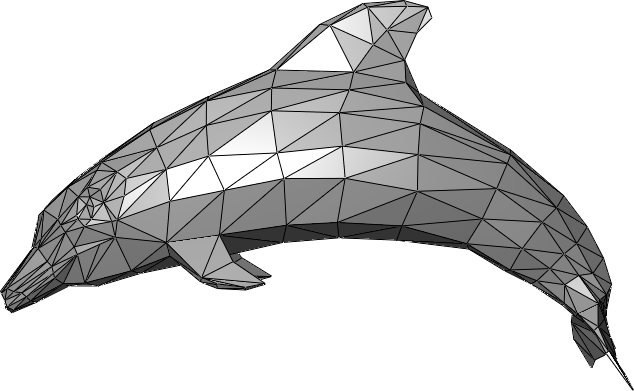
\psfig{file=Dolphin_triangle_mesh.png,width =3in}
\caption{A simple scene containing a dolphin constructed from triangle primitives~\cite{wiki:mesh}.}
\label{fig:dolphin}
\end{figure}

\begin{figure}
\centering

\psfig{file=Glasses_800_edit.png,width =3in}
\caption{A ray traced scene featuring shadows on the wall and beneath the glasses, reflections on the glossy surfaces of the glasses, and refractions through the glass stems and ice cube~\cite{wiki:rayTracing}.}
\label{fig:glasses}
\end{figure}

Since many rays of light from a light source may not ultimately reach the viewer, it is more practical to start from the viewer and trace paths of light backwards. For every pixel on a display, a ray is traced from the viewer through the pixel and into the 3D scene. When a ray intersects with an object in the scene it can recursively generate more rays in directions that will contribute to an appearance of reflections, refrations, or shadows~\cite{Whitted:1980}. While ray tracing can create highly realistic images, the process of tracing a large number of rays for a 3D scene with many primitives on a high resolution display can take a very long time.

Ray tracing a single frame of a 3D scene can involve testing for intersections of billions of rays against millions of primitives such as triangles. In order to speed up this process, acceleration data structures can be used to organize the primitives by their location so that only a small subset of them need to be tested for intersection against any given ray. Acceleration data structures usually take the form of a tree: the top node represents the entire 3D volume of the scene and the children of every node divide up the volume of their parent node into subsections. Although these acceleration data structures speed up ray intersection testing, the time it takes to build these trees can negatively impact performance. This is especially apparent in scenes with moving objects since the acceleration data structures need to be rebuilt or updated to accurately reflect the new locations of objects~\cite{Karras:2012}.

The research discussed here addresses methods for building and maintaining acceleration data structures in a way that minimizes the combined time spent constructing the data structure and using it to test for ray intersections. In particular, parallel computing on the GPU can be effectively utilized to decrease the time spent on an acceleration data structure. More efficient acceleration data structures allow for ray tracing scenes with motion in real time.

\begin{figure}
\centering
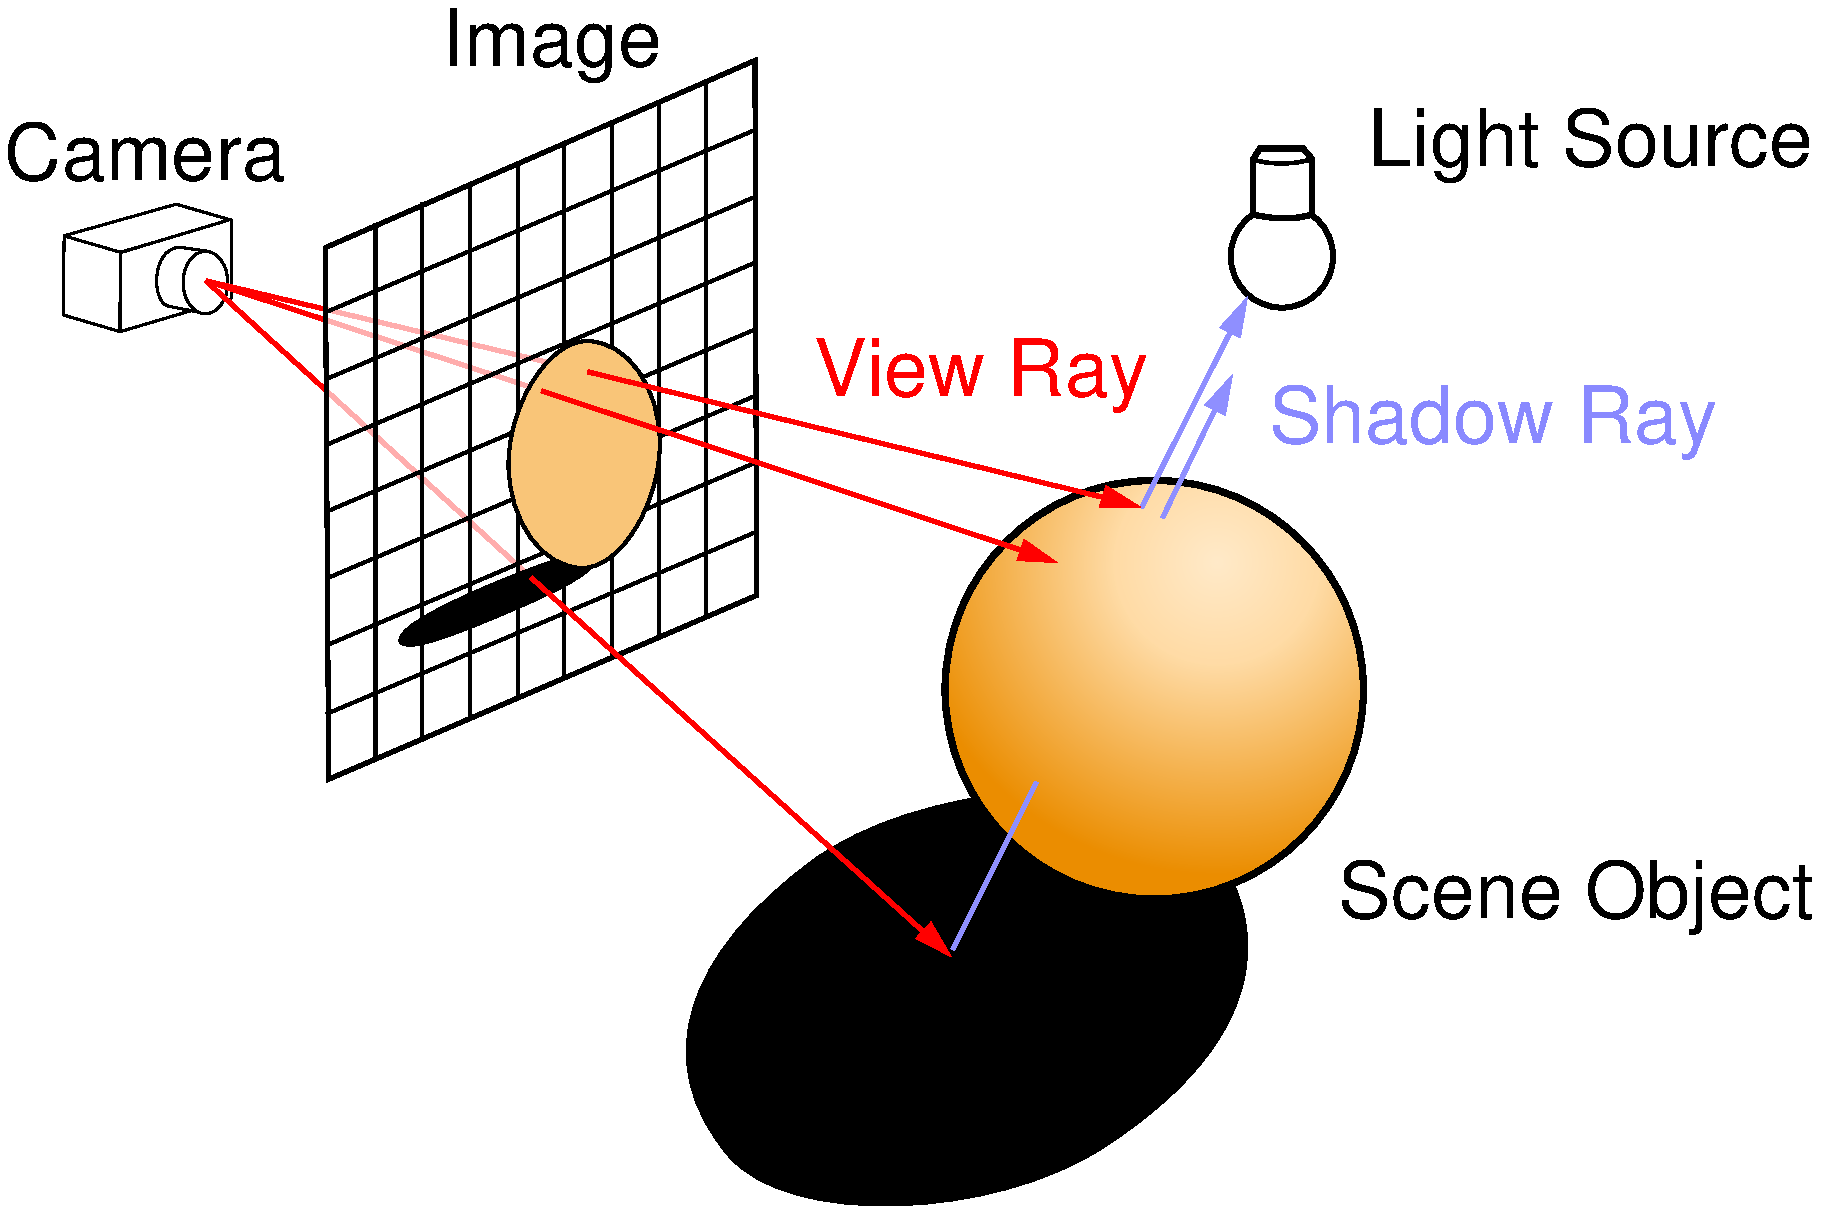
\psfig{file=Ray_trace_diagram.pdf,width =3in}
\caption{A ray is cast through every pixel of the image plane and tested for intersection with objects in the scene. When intersections occur, the angle of reflection is calculated and a new ray is sent out. Eventually, if a ray intersects with a light source, the color information propagates back to the pixel~\cite{wiki:rayTracing}.}
\label{fig:ray_diagram}
\end{figure}

\begin{figure}
\centering
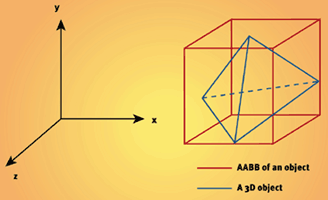
\psfig{file=aabb.png,width =3in}
\caption{An axis aligned bounding box containing an object constructed from four triangles. Note that the box is fitted as tightly as possible and the edges of the box lie parallel to the axes of the scene.}
\label{fig:AABB}
\end{figure}

% From http://gimpact.sourceforge.net/manual/manual_figures/aabb.gif

\begin{figure*}
\centering
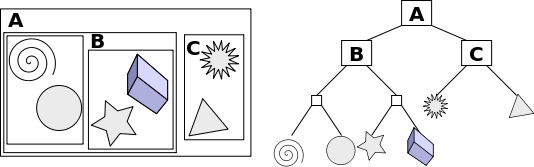
\psfig{file=BVH.png,width =6in}
\caption{Left: A 2D scene with rectangles as bounding boxes. Right: One possible BVH configuration for the 2D scene. Note that each internal node has exactly two children and that objects that are close in the scene are also close in the BVH tree~\cite{wiki:bvh}.}
\label{fig:BVH}
\end{figure*}

\todo[inline]{Needs more work}

\section{Acceleration Data Structures}
\label{sec:body}

If primitives of a scene are stored in a data structure that helps identify where they are located in the scene, then a ray only needs to check for intersections with objects located in the parts of the scene the ray is passing through. This can drastically improve the performance of intersection testing for each ray~\cite{wiki:rayTracing}.

A common way to make intersection tests easier to calculate is to surround primitives with bounding boxes. A bounding box is just a box that completely contains an object as tightly as possible. A common approach is to use \emph{axis-aligned bounding boxes} (AABBs), which are aligned with the axes of the scene as a whole. It is usually much simpler to test for ray intersections with AABBs than with the objects they contain. If a ray does not intersect with an object's AABB, then it cannot intersect with the object itself. However, if it does intersect with the AABB, then a more costly check must be made to test for intersection with the contained object. Overall, the use of AABBs can reduce the cost of testing for intersections since a ray misses many more objects than it hits~\cite{wiki:box}.

\emph{Bounding volume hierarchies} (BVHs) extend the idea of AABBs to a tree-like data structure. The root node of a BVH is an AABB that contains the entire scene. The child nodes of any parent node subdivide the total volume of the parent node into multiple smaller sub-volumes. By continually separating volumes into smaller volumes, it becomes possible to group close primitives together. The lower nodes on the tree give more precise location information than the higher nodes. As opposed to other types of acceleration data structures, BVHs define the volumes by the objects they contain rather than splitting volumes and then determining which objects should go in each node. Therefore, an object would never be in more than one node~\cite{wiki:bvh}.

Searching for a ray intersection with objects in a BVH occurs in a top-down manner. First, the ray is tested against the root of the node to check if it even intersects with the scene. If it does, then each of the root's children is checked for intersection. Any child node that the ray misses can be entirely eliminated from the rest of the search, since the objects contained entirely within the node will also not intersect. Ray tracing with a BVH structure can therefore greatly reduce the number of intersection checks performed per ray~\cite{wiki:bvh}.

\todo[inline]{Needs more work}

\section{BVH Construction}
\label{sec:bvh}

In order to speed up the construction of BVHs for real-time ray tracing, Tero Karras has developed a method for constructing an entire BVH tree in parallel on a GPU. The method follows a series of four main steps. The method first assigns a value called a \emph{Morton Code} to each primitive based upon its location in the scene. The Morton codes are then sorted. Next, a \emph{binary radix tree} is constructed in parallel, which arranges close primitives near each other in the tree. The last step fits an AABB around the contents of each node in the binary radix tree in parallel to form the final BVH~\cite{Karras:2013}. The next sections will cover each of these steps in more detail.

\subsection{Morton Codes}
\label{sec:mortonCodes}

The location of each primitive in the scene can be represented by the $x$, $y$, and $z$ coordinates of its AABB. The Morton code of a primitive combines the coordinates into a single value by interleaving the binary representations of the $x$, $y$, and $z$ coordinates. A Morton code has the form \begin{math}X_{0}Y_{0}Z_{0}X_{1}Y_{1}Z_{1}\dots\end{math} where the $x$ coordinate is represented in binary as \begin{math}X_{0}X_{1}X_{2}\dots\end{math}, and similarly for the $y$ and $z$ coordinates~\cite{Karras:2012}.

Figure~\ref{fig:MortonCodeFigure} shows a two dimensional scene area with the Morton codes of each coordinate location. The lowest valued Morton code appears in the upper-left corner of the scene where both coordinates are zero. The zig-zag pattern on the image shows the sequence of increasing Morton codes, which ultimately ends with the highest value in the lower-right corner. After each primitive is assigned a Morton based on its location, all of the Morton codes are sorted~\cite{Karras:2012}.

Note that all codes that start with a 0 bit are located in the upper half of the scene, and within that section all codes that have a 0 as the second bit are located on the left half of that section. This property of Morton codes will allow primitives that are near each other to have long common prefixes between their Morton codes, which will prove to be important for the binary radix tree construction.

\begin{figure}
\centering
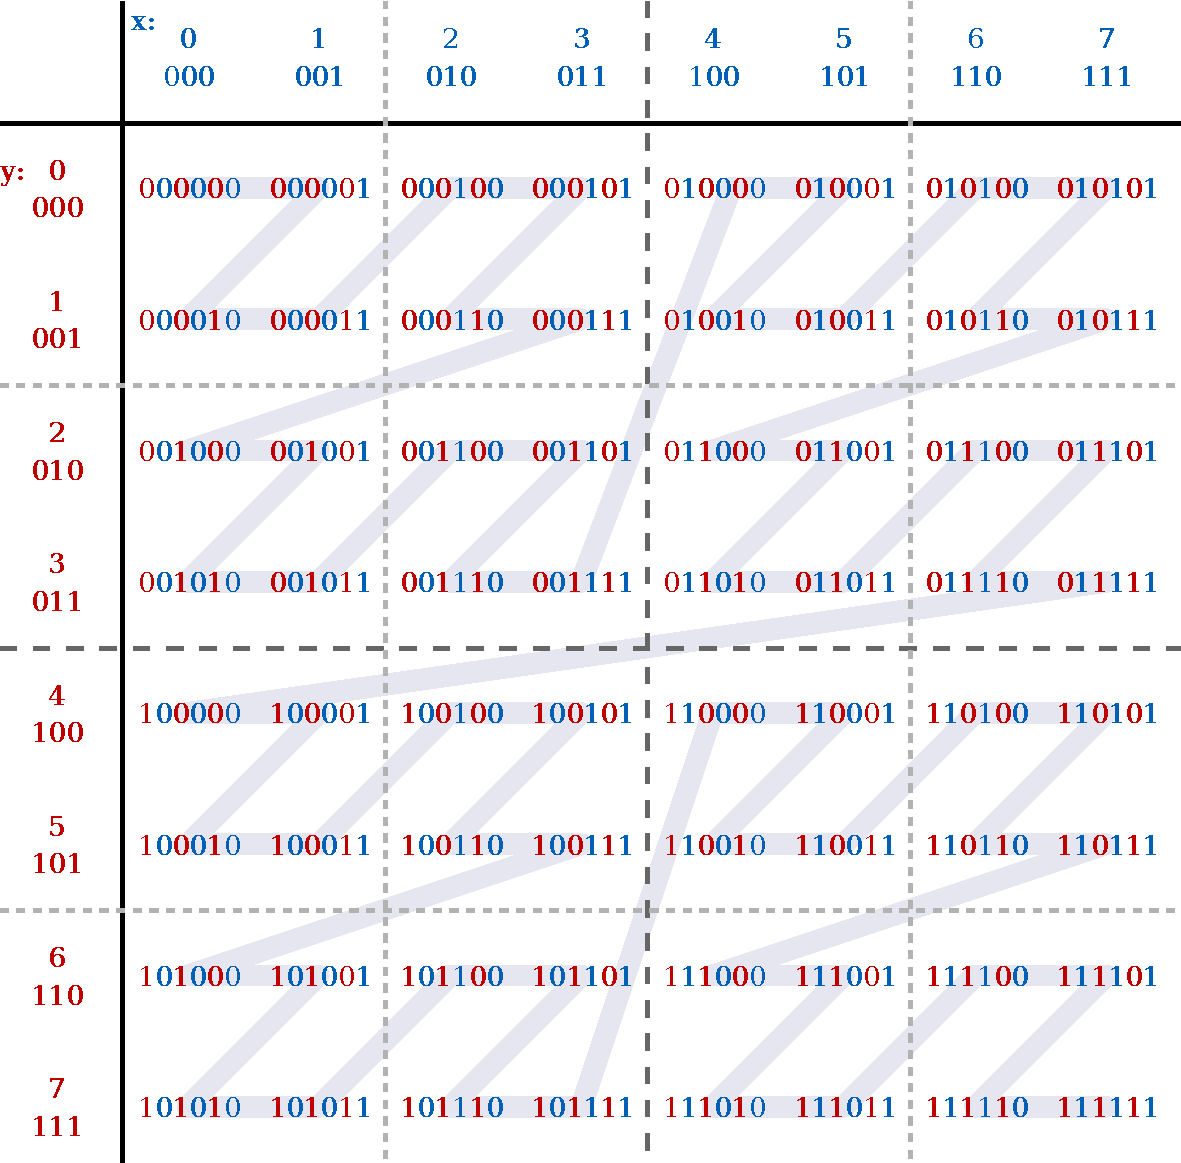
\psfig{file=Z-curve.pdf,width =3in}
\caption{Morton codes for each location in a 2D scene. Notice that each Morton code is made by interleaving the bits of the $x$ (blue) and $y$ (red) coordinates for its location~\cite{wiki:morton}.}
\label{fig:MortonCodeFigure}
\end{figure} 

\subsection{Binary Radix Tree Construction}
\label{sec:brts}

\subsubsection{Binary Radix Tree Fundamentals}
\label{sec:brtFundamentals}

The array of sorted Morton codes can be thought of as a set of $n$ bit string keys \begin{math}k_{0},\dots,k_{n-1}\end{math} where $n$ represents the number of primitives in the scene. A binary radix tree organizes the keys into a tree structure where the internal nodes represent common binary prefixes of the keys. Figure~\ref{fig:BinaryRadixTree} shows an example of the binary radix tree for a set of eight binary keys, which would be the Morton codes of primitives in a scene. Each key is a leaf node, and each internal node represents the longest common prefix shared by all the keys under it. Every internal node always has exactly two children: the left child has the common prefix of the parent followed by a 0 bit, and the right child has the same common prefix but followed by a 1 bit. Since every internal node has exactly two children, a binary radix tree with $n$ leaf nodes will always have exactly $n-1$ internal nodes~\cite{Karras:2012}.

Every key in a binary radix tree must be unique, but duplicate Morton codes could exist from the primitives in the scene. To ensure uniqueness, the binary representation of each key's index can be concatenated onto the end of the key. These concatenations do not need to be stored, but can be performed as needed when comparing identical keys~\cite{Karras:2012}.

\begin{figure}
\centering
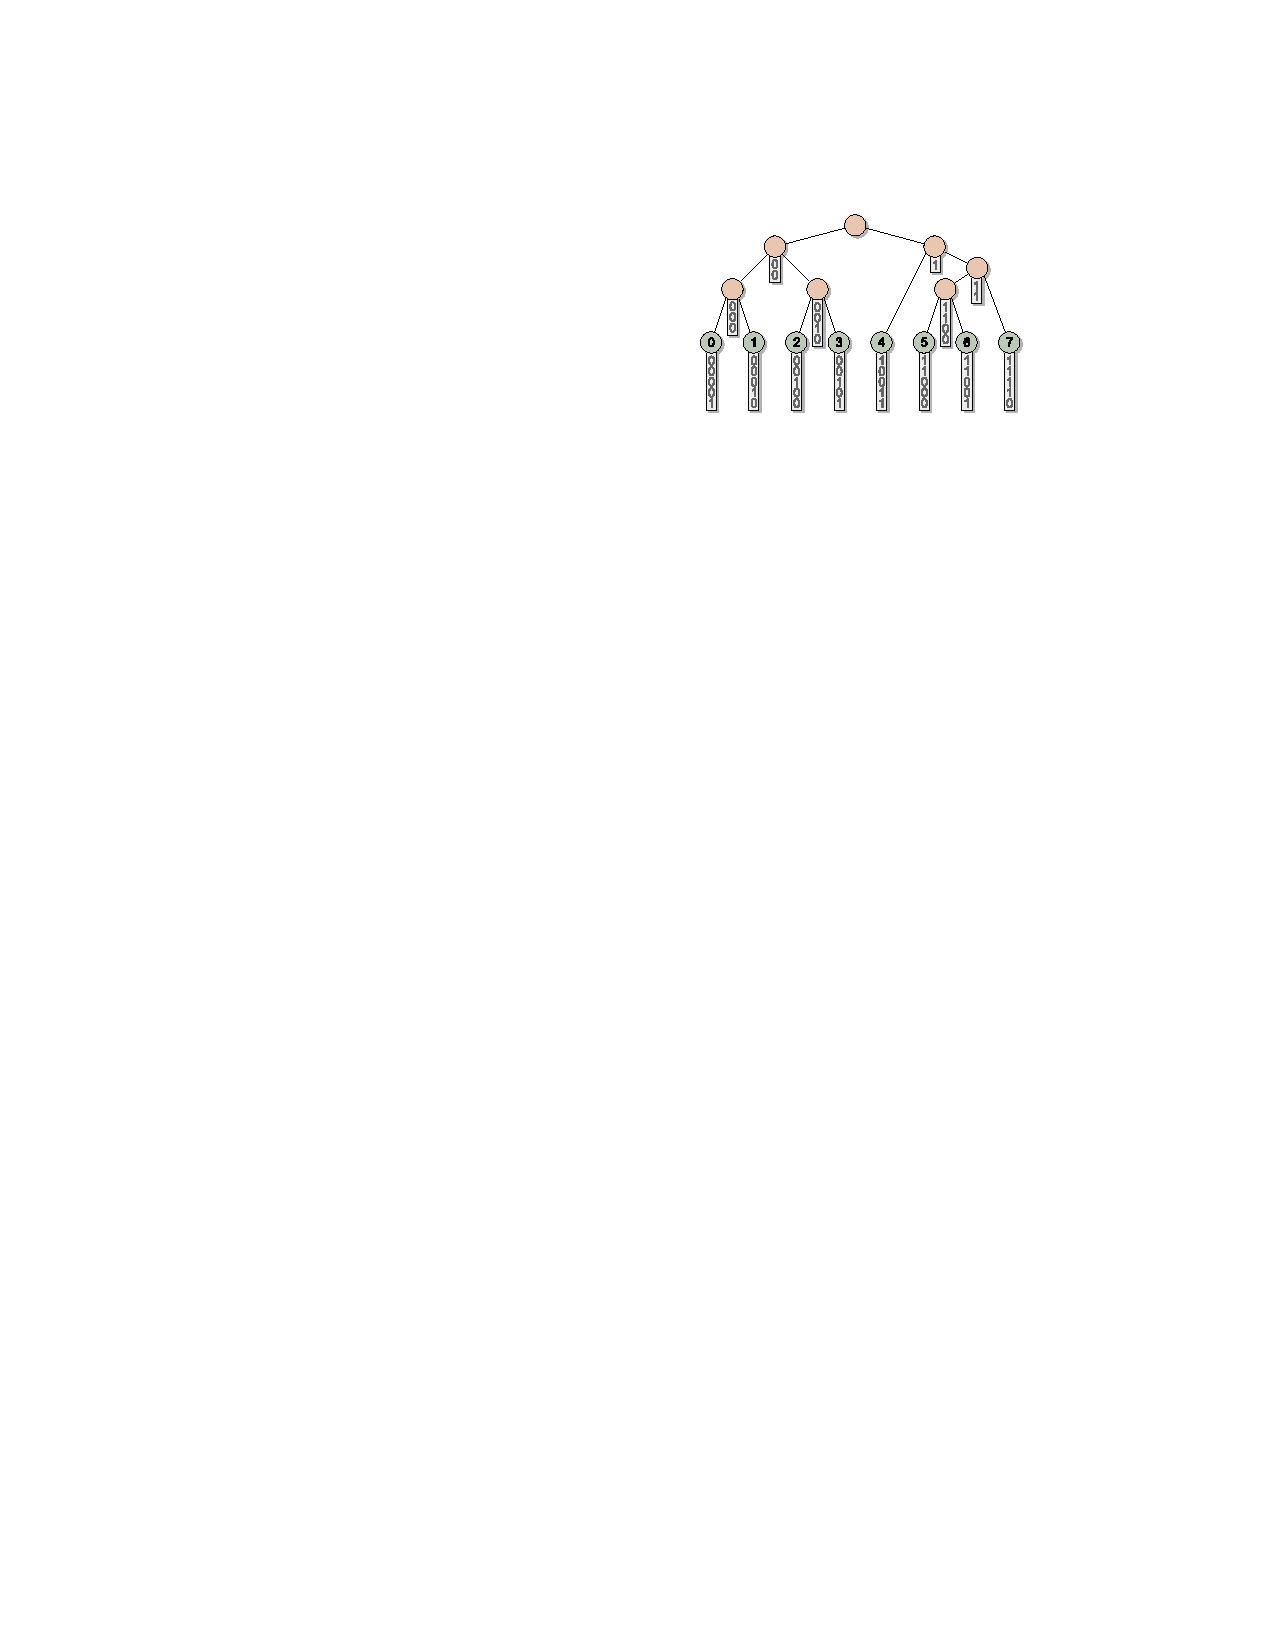
\psfig{file=BinaryRadixTree.pdf,width =3in}
\caption{An ordered binary radix tree. There are eight leaf nodes containing 5-bit keys which appear in lexicographical order. Each internal node covers a linear range of keys with a common prefix, which is displayed directly beneath the node. The range of keys covered by an internal node is partitioned into two ranges according to their first differing bit; the two subranges are represented by the two children of the internal node~\cite{Karras:2012}.}
\label{fig:BinaryRadixTree}
\end{figure}

\subsubsection{Binary Radix Tree Properties}
\label{sec:brtProperties}

In order to process every internal node of the binary radix tree in parallel, it must be possible to determine several properties about a node. These properties include the range of keys that a node covers, the length of the longest common prefix of those keys, and what the node's children are. Additionally, these must be determined without depending on the work done in any other internal nodes since all the nodes will be working in parallel. The following discussion will cover these important properties.

The keys covered by an internal node can be represented as a linear range $[i,j]$. Using Figure~\ref{fig:BinaryRadixTree} as an example, the root node covers keys 0 through 7, so it can be represented as the range $[0,7]$. Its left child can be represented as $[0,3]$ and its right child as $[4,7]$.

The length of the longest common prefix between two keys $k_{i}$ and $k_{j}$ is denoted by $\delta(i,j)$. For example, the longest common prefix between key 0 and key 3 in Figure~\ref{fig:BinaryRadixTree} is "00", which has a length of two digits. So $\delta(0,3)$ is 2.

The prefix for each node can be determined by solely inspecting the first and last key in its key range. This is because all keys between the first and last key will also share the same prefix since all keys are in lexicographical order~\cite{Karras:2012}. As an example, the left child of the root in Figure~\ref{fig:BinaryRadixTree} covers keys 0 through 3. By only looking at keys 0 and 3, it can be determined that they share the prefix "00". All keys between 0 and 3 will also have the prefix "00", otherwise they would not fall in that range.

An internal node partitions its range of keys into two subranges for its children according to the first differing bit among the keys. For example, the left child of the root in Figure~\ref{fig:BinaryRadixTree} covers keys 0 through 3 with a common prefix of "00". This node will divide its keys among its children based on the value of the 3rd bit of the keys, since the 3rd bit comes directly after the common prefix. All keys in the range with 0 as the 3rd bit will belong to the left child and the keys with 1 as the 3rd bit will belong to the right child. The index of the last key where the differing bit is 0 is called a \emph{split position}, and is denoted by $\gamma$. If the range of keys covered by a node is $[i,j]$, then the split position can be anything from $i$ to $j-1$. The split position cannot occur at $j$, since the differing bit must be a 1 for key $j$. The split position for the left child of the root in Figure~\ref{fig:BinaryRadixTree} is 1 because key 1 is the last key in the range $[0,3]$ with the prefix "000", and the next key must have the prefix "001"~\cite{Karras:2012}. The subrange $[i,\gamma]$ represents the range of keys covered by the left child and the subrange $[\gamma+1,j]$ represents the range covered by the right child.

For an internal node with range $[i,j]$, the equality $\delta(\gamma,\gamma+1) = \delta(i,j)$ always holds true and is important for finding the the split position. In fact, $k_{\delta}$ and $k_{\delta+1}$ is the only pair of adjacent keys in the range where the prefix length of the pair is equal to the prefix length of the range. Pairs of adjacent keys to the left of the split position will have a longer common prefix than the range since they all have 0 in the differing bit position. Adjacent keys to the right of the split position are analogous, but with all having a 1 in the differing bit position.

\subsubsection{Setup for Binary Radix Tree Construction}
\label{sec:setup}

It is possible to construct a binary radix tree by starting with root node, finding the first differing bit in the keys, creating the child nodes, then handling each child recursively. However, this is not parallel because a node can not be started until all of its ancestors have been processed. Parallel construction can be achieved by creating a connection between node indices and keys through a particular tree setup. This is done by assigning indices to internal nodes in a way that enables finding their children without depending on that node's ancestors being complete~\cite{Karras:2012}.

\begin{figure}
\centering
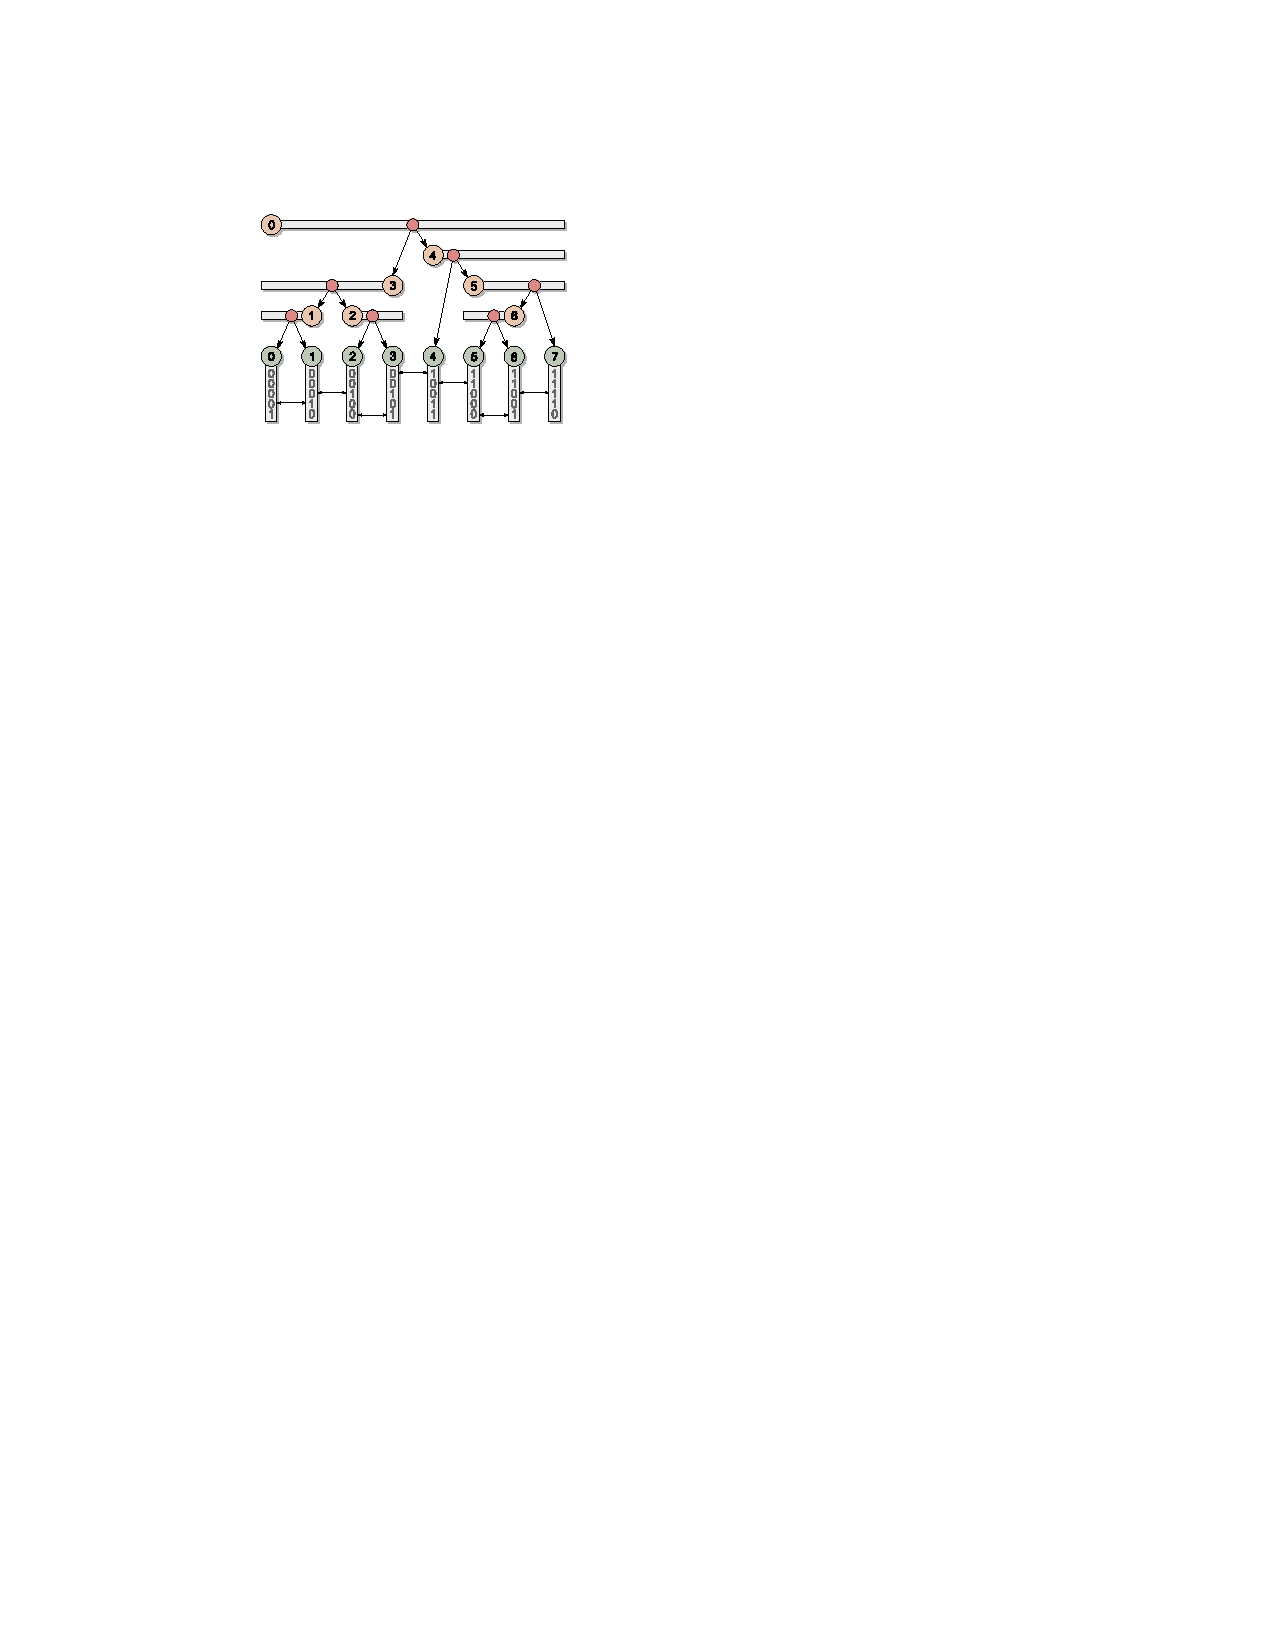
\psfig{file=radix_tree_arrays.pdf,width =3in}
\caption{This figure shows the storage locations of nodes for the binary radix tree displayed in Figure~\ref{fig:BinaryRadixTree}. The internal nodes have been assigned indices from 0 to 6 and are lined up with leaf nodes with the same indices. The range of keys covered by each internal node is shown as a horizontal bar, and a red circle lies immediately after each node's split position~\cite{Karras:2012}.}
\label{fig:BinaryRadixArrays}
\end{figure}

Figure~\ref{fig:BinaryRadixArrays} presents a visual representation of how the nodes of the binary radix tree from Figure~\ref{fig:BinaryRadixTree} will be stored. The leaf nodes and internal nodes are stored in two separate arrays, $L$ and $I$, respectively. The root will always be located at $I_{0}$. The children of internal nodes are placed at an index according to the internal node's split position. The left child is located at $L_{\gamma}$ if it is a leaf, or at $I_{\gamma}$ if it covers more than one key. Similarly, the right child is located at $L_{\gamma+1}$ or $I_{\gamma+1}$~\cite{Karras:2012}. For example, the split position of the root in Figure~\ref{fig:BinaryRadixArrays} is at index 3, so its left child is stored in $I_{3}$ and its right child is stored in $I_{4}$.

It is important to note that the index of every internal node is equal to the index of either its first or last key. The index of a node will be equal the index of its first key if the node is a right child of its parent. Figure~\ref{fig:BinaryRadixArrays} shows that internal node 4 is a right child of the root, that its index coincides with it first key (key 4), and that its range extends rightward. Conversely, internal node 3 is a left child of the root, its index coincides with its last key (key 3), and its range extends leftward. More generally, if a node covers the range $[i,j]$, then its left child will be located at $\gamma$, which is the end of its range $[i,\gamma]$. The right child will be located at $\gamma+1$, which is the beginning of its range $[\gamma+1,j]$~\cite{Karras:2012}.

\subsubsection{Construction Algorithm}
\label{sec:algorithm}

The goal of the construction algorithm is to determine the range of keys covered by each internal node, as well as the indices of its children. One end of the range is given by the internal node's index, and the other end of the range can be found by examining the surrounding keys. The indices of the children can be found by finding the split position. Because of all of the previous setup, each internal node can be processed independently and in parallel with the other internal nodes~\cite{Karras:2012}.

Consider processing an internal node $i$, which is in the $i$th position of the array $I$. For a concrete example consider $i$ is 2, which can be seen to cover keys 2 through 3 in Figure~\ref{fig:BinaryRadixArrays}. First, the key $k_i$ is compared with its neighbors $k_{i-1}$ and $k_{i+1}$ to determine the direction of the range (to the left or to the right). If the prefix between $k_i$ and $k_{i-1}$ is longer than the prefix between $k_i$ and $k_{i+1}$, then the direction of the range extends to the left, otherwise the range extends rightward. In the example, $\delta(2,3) = 4$ while $\delta(2,1) = 2$, so the range of node 2 extends to the right since it shared a longer common prefix with its right neighbor. Let $d$ be $+1$ if the range extends rightward, and $-1$ if the range extends leftward ~\cite{Karras:2012}.

The next task is to determine $j$, which represents the index of the other end of the range $[i,j]$. For the example, $j$ is 3 since the range of the node at index 2 extends from index 2 to index 3. Every internal node covers at least two keys, so $k_i$ and $k_{i+d}$ must belong to $I_i$. The other neighboring key $k_{i-d}$ must belong to $I_{i-d}$. The two keys $k_i$ and $k_{i+d}$ share a common prefix that is different and longer than the prefix between $k_i$ and $k_{i-d}$. Let $\delta_{min}$ represent the value of $\delta(i, i-d)$. In the example, $\delta_{min}$ equals 2, with the common prefix being "00". The value of $\delta_{min}$ is equivalent to the length of the prefix represented by the parent of the node currently under consideration. This fact is used to determine the index of $j$. For any $k_m$ belonging to $I_i$, the inequality $\delta(i,m)>\delta_{min}$ always holds true. Therefore, $\delta_{min}$ gives a lower bound for the length of the prefix for the section of keys covered by $I_i$. So the index $j$ marking the other end of the range can be found by searching for the largest $l$ that satisfies $\delta(i, i+ld)>\delta_{min}$~\cite{Karras:2012}.

Finding $j$ is achieved by first finding a power-of-two upper bound for $l$, denoted as $l_{max}$. Then $l$ can be found by using binary search in the range $[0,l_{max}-1]$. These two steps will be discussed next.

To determine $l_{max}$, which is the exclusive upper bound for $l$, $l_{max}$ will start at 2 and continue to double until it no longer satisfies the inequality $\delta(i,i+l_{max} \cdot d)>\delta_{min}$. For example, in $I_5$, $\delta_{min}$ is 1 with the prefix "1". Start with $l_{max}=2$. The prefix length $\delta(5, 5+2 \cdot 1)$ is 2, which is still greater than $\delta_{min}=1$ so $l_{max}$ should be doubled to become 4. Now the prefix length $\delta(5, 5+4 \cdot 1)$ is $\delta(5,9)$. Whenever an argument to the $\delta$ function is out of bounds, the function should return -1. Since -1 is not greater than $\delta_{min}=1$, the search for $l_{max}$ is finished with $l_{max}=4$. We can see from Figure~\ref{fig:BinaryRadixArrays} that $l$ is 2 for node 5 since it covers the keys $[5,5+2]$. Therefore, $l_{max}=4$ is the correct exclusive power-of-two upper bound for node 5~\cite{Karras:2012}.

Once the upper bound $l_{max}$ is determined, $l$ can be found by using binary search in the range $[0,l_{max}-1]$. The goal is to find the largest $l$ such that $\delta(i,i+l \cdot d)$ is greater than $\delta_{min}$. The value of $j$ is then determined by $i+l \cdot d$. Consider $l$ as an unsigned binary number. Note that if $l_{max}$ is 4, $l$ can be a 2-bit number since the maximum value it could be is 3. Similarly, if $l_{max}$ is 8, $l$ can be a 3-bit number, since its maximum value is 7. To determine $l$, consider each bit of $l$ in turn, starting with the highest bit, and set it to one unless the new value of $l$ fails to satisfy the inequality $\delta(i,i+l \cdot d)>\delta_{min}$~\cite{Karras:2012}. Essentially, this is identical to looping through the range \{$l_{max}/2, l_{max}/4,\dots, 1$\}, setting each value to $t$ and increasing $l$ by $t$ only if the inequality $\delta(i,i+(l+t) \cdot d)>\delta_{min}$ holds. For example, for node 5, with $\delta_{min}=1$ and $l_{max}=4$, the loop goes through the range \{$2, 1$\}, which makes sense since $l$ must be a 2-bit number. $l$ starts at 0. The value of $\delta(5, 5+(0+2) \cdot 1)$ is 2, which is greater than $\delta_{min}=1$, so $l=l+2$. Now $l$ is 2 for the next iteration of the loop and $t$ is 1. The value of $\delta(5, 5+(2+1) \cdot 1)$ is -1 since the index of 8 is out of range, so nothing is added onto $l$ for this iteration. The loop is done and $l$ has the value of 2. Now $j$ can be determined by the formula $j=i+l \cdot d$, which is 7 for node 5. This is correct since node 5 covers the range $[5, 7]$.

Now that the range of keys for the node has been determined, the length of the common prefix of those keys, denoted by $\delta_{node}$, is calculated as $\delta(i,j)$. The next step of the algorithm is to determine the split position $\gamma$, which can be done using binary search.

To find $\gamma$, the goal is to determine the largest $s$ in the range $[0, l-1]$ that satisfies $\delta(i, i+s \cdot d) > \delta_{node}$. Specifically, the goal is to determine the last index in the range of keys where the first differing bit of the key is 0~\cite{Karras:2012}.

This binary search is very similar to the previous one. If $l$ is 3 or 4, $s$ needs 2 bits to represent the values 2 or 3. Similarly, if $l$ is 5, 6, 7, or 8, then $s$ needs 3 bits to represent the values from 4 to 7. $s$ starts at 0. The loop sets the variable $t$ to each value in the range \{$ciel(l/2), ciel(l/4), \dots, 1$\}. Then if $\delta(i, i+(s+t) \cdot d)>d_{node}$, $s$ is increased by $t$. For example, consider node 5, which has $l=2$ and $d_{node}=2$. The loop will go over the range \{$1$\}. For this single iteration the value of $t$ is 1 and $\delta(5, 5+(0+1) \cdot d)$ is 4, which is greater than $d_{node}=2$ so $s$ becomes 1~\cite{Karras:2012}.

Now that $s$ is known, $\gamma$ is determined by $i + s \cdot d + min(d, 0)$. The  addition by $min(d, 0)$ serves to place $\gamma$ in the left half if the range was extending to the left. In that case, $i + s \cdot d$ gets us to $\gamma + 1$ instead of $\gamma$, since we are effectively scanning from right to left. For node 5, $\gamma=5+1+0=6$, which matches Figure~\ref{fig:BinaryRadixArrays}.

Lastly, the node needs to store its child pointers. If $min(i,j)=\gamma$ then the left part is solely $\gamma$, so the left child should be the leaf $L_{\gamma}$. Otherwise, the left child should be the internal node $I_{\gamma}$. If $max(i,j)=\gamma+1$ then the right  part is solely $\gamma+1$, so the right child should be the leaf $L_{\gamma+1}$. Otherwise, the right child should be the internal node $I_{\gamma+1}$. In summary, given $i$, $j$, and $\gamma$, the left child of $I_i$ covers the range $[min(i,j), \gamma]$ and the right child covers the range $[\gamma+1,max(i,j)]$. If there is only one key in a range, then the child is a leaf, otherwise it is an internal node.

Overall, on the GPU, each thread is responsible for only one internal node.

\subsubsection{Time Complexity}
\label{sec:time}

For a node that covers $q$ keys, each of the three loops above executes at most $ciel(log_{2}(q))$ iterations. Since $q$ is lesser than or equal $n$ for all $n-1$ internal nodes, the worst-case time complexity for the entire tree is $O(n log n)$. The worst case occurs when the height of the tree grows proportional to n, but this is unlikely since the height of the tree is limited to the length of the keys~\cite{Karras:2012}.

\subsection{Fitting AABBs}
\label{sec:fitting}

To turn the binary radix tree into a BVH, one simply need to surround the contents of each node with an AABB. To do this in parallel, each thread should start from a leaf node and travel up the tree from there. However, each internal node has two children and it should not be processed twice. Therefore, each internal node keeps an atomic count of how many threads have visited it. The first thread that reaches an internal node terminates immediately, while the second thread gets to process the node~\cite{Karras:2012}.

%
%\begin{figure*}
%\centering
%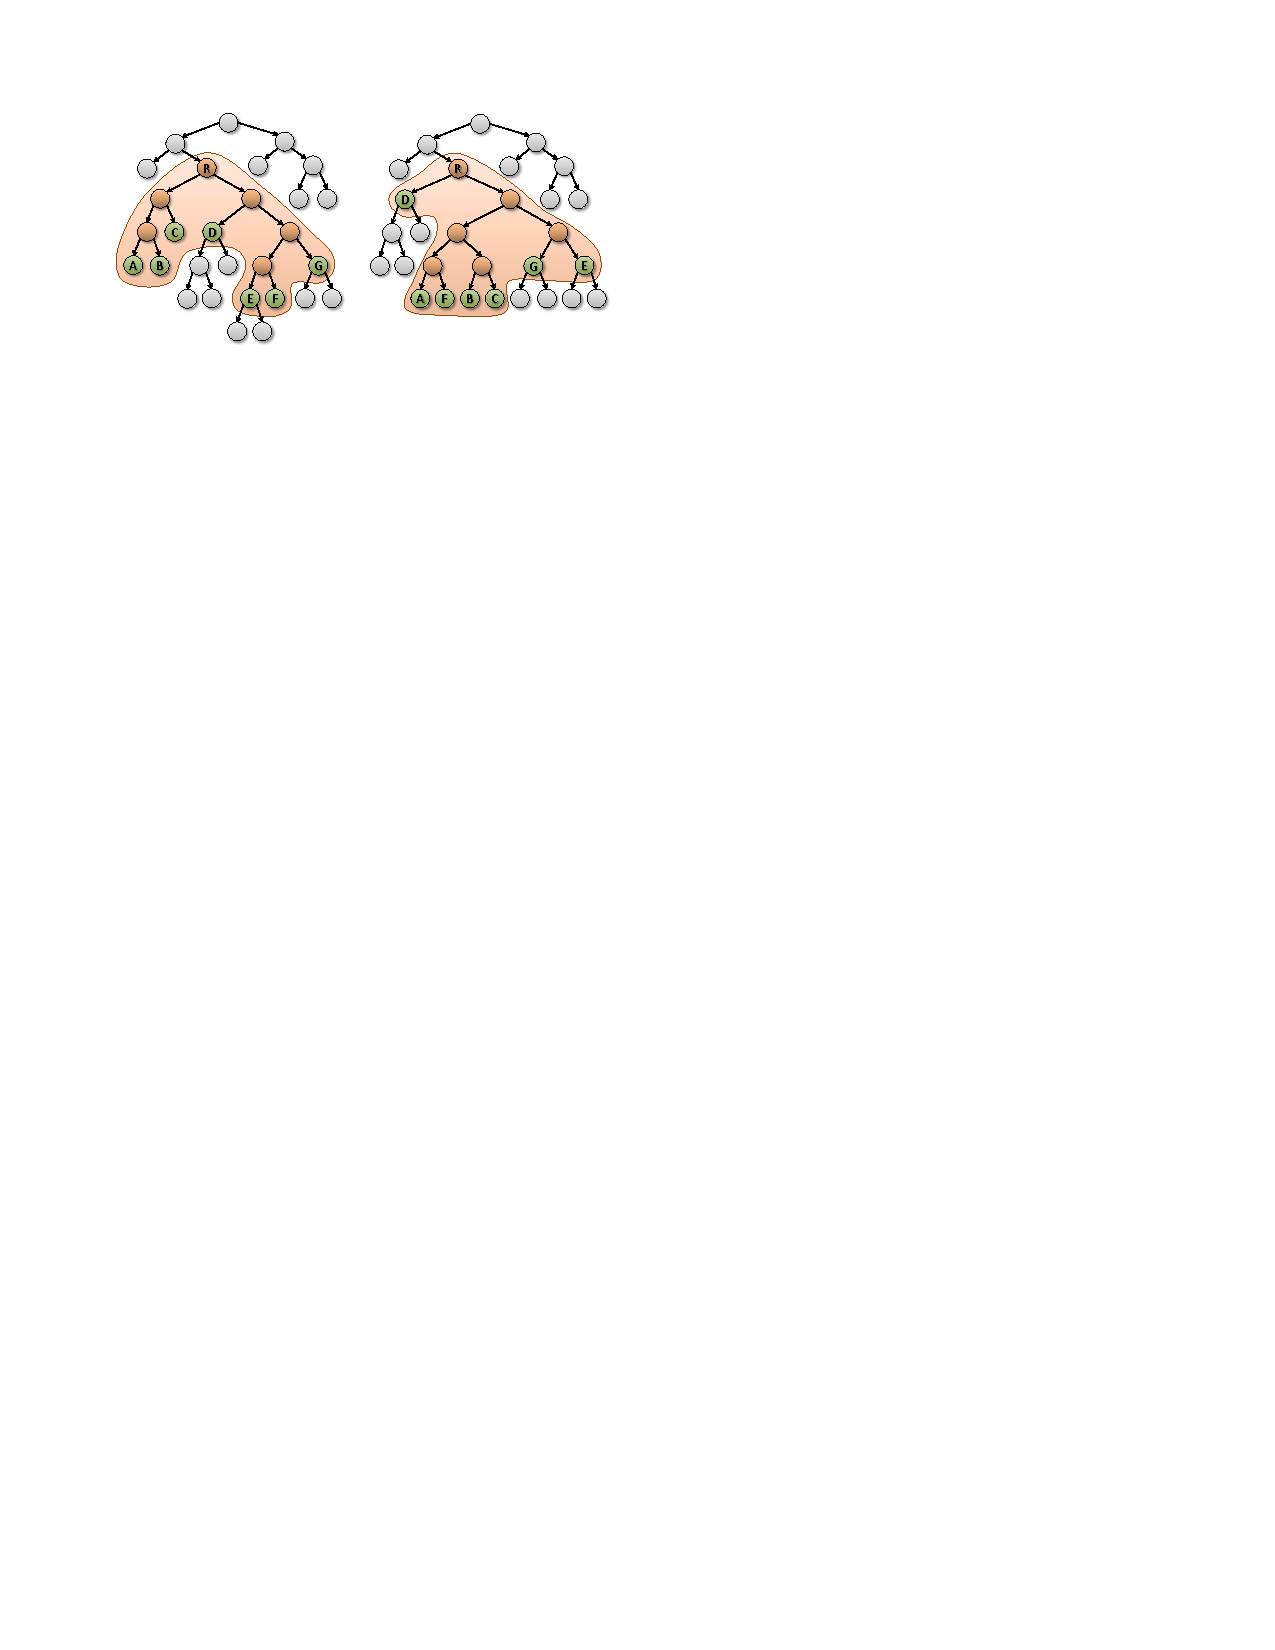
\psfig{file=tree.pdf,width =6in}
%\caption{A treelet rotation that decreases the ray tracing cost of the BVH~\cite{Karras:2013}.}
%\label{fig:treelet}
%\end{figure*}

%\begin{figure*}
%\centering
%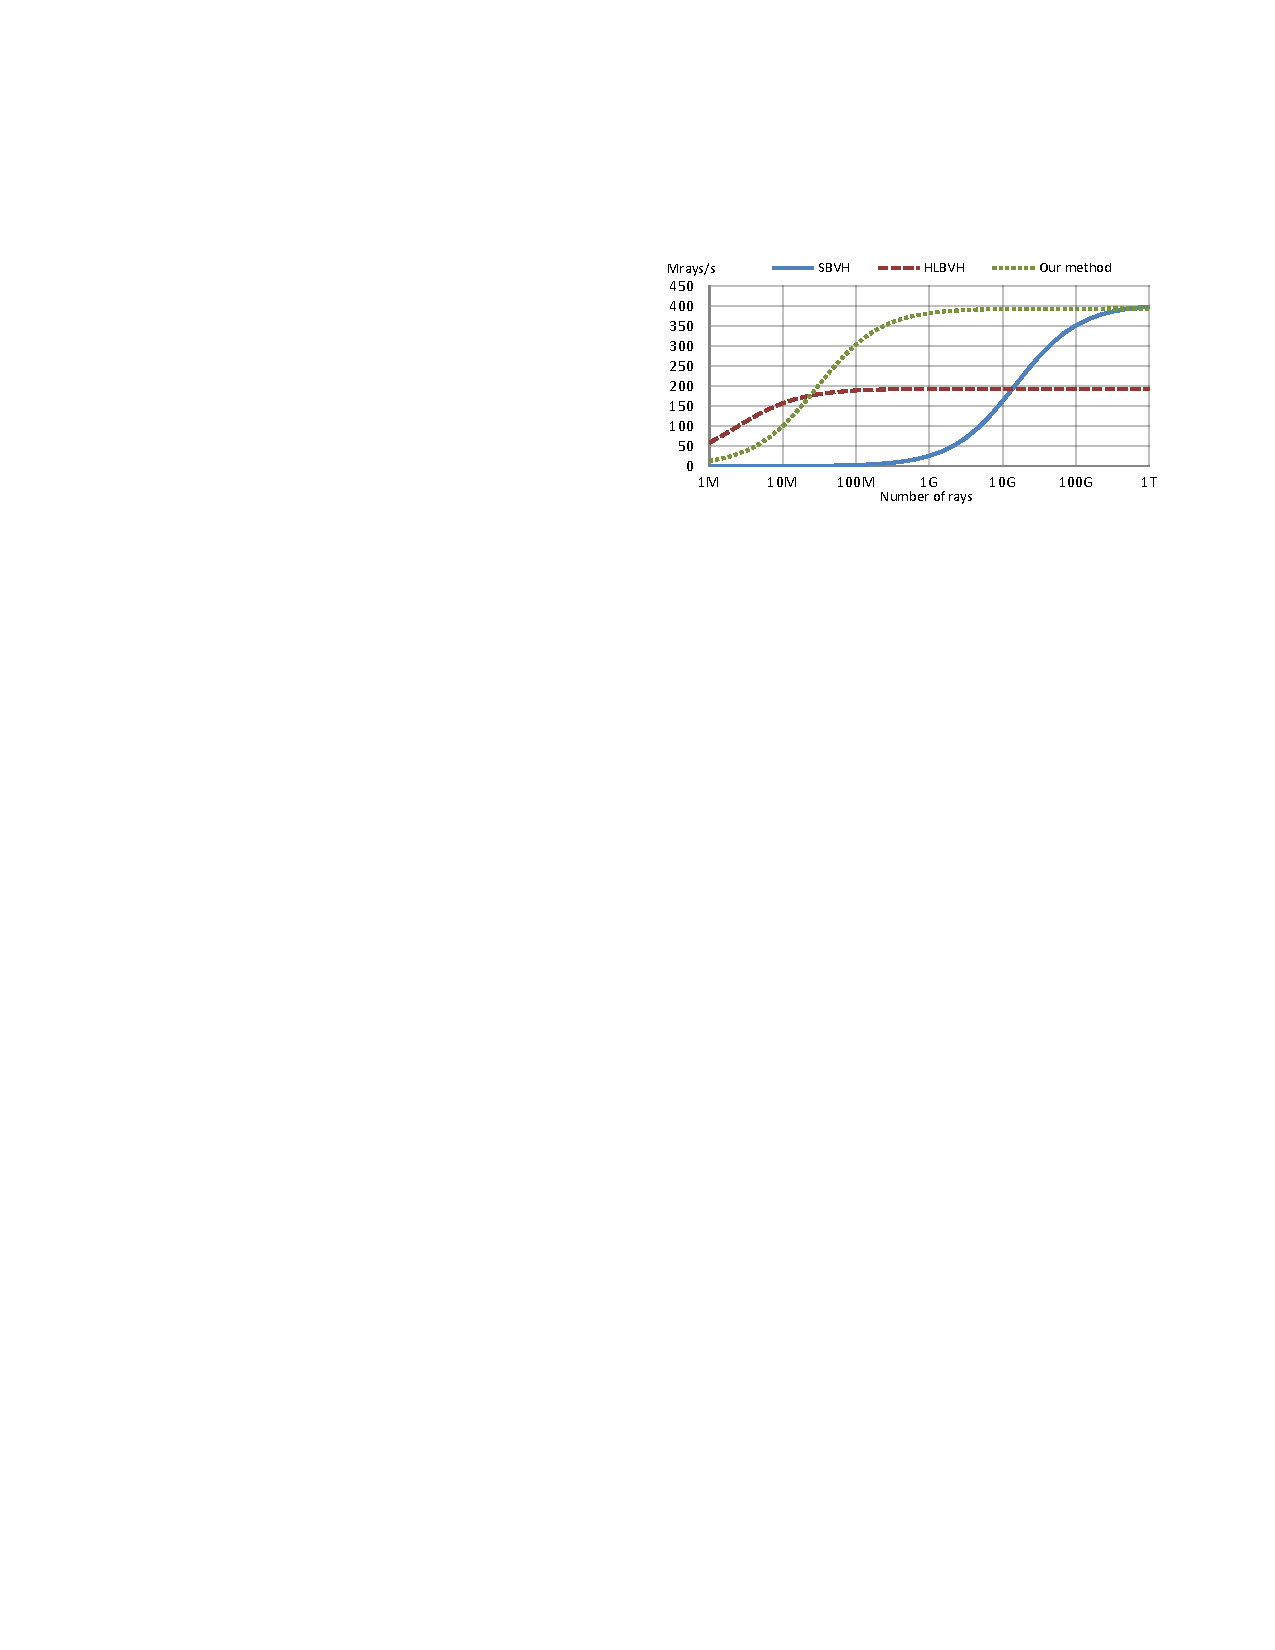
\psfig{file=graph.pdf,width =6in}
%\caption{Performance comparison from primary source~\cite{Karras:2013}.}
%\label{fig:treeletPerformance}
%\end{figure*}

%\todo[inline]{Needs more work}

\section{Conclusion}
\label{sec:conclusion}

As shown in Figure~\ref{fig:RadixCores}, the performance of the algorithm scale well as the number of cores increase. The execution time is inversely proportional to the number of cores. This is an excellent quality because it means that the performance can be roughly doubled by doubling the number of cores assigned to the task~\cite{Karras:2012}.

Figure~\ref{fig:RadixPerformance} shows a comparison between this algorithm and the best previously known algorithm by Garanzha et al. It is apparent that the algorithm presented runs nearly twice as fast as the previous best. Additionally, the construction time is dominated by the sorting of primitives (shown as light green) rather than the hierarchy generation or AABB calculation. Conversely, the other algorithm appears to spend most of its time performing hierarchy generation.

\begin{figure}
\centering
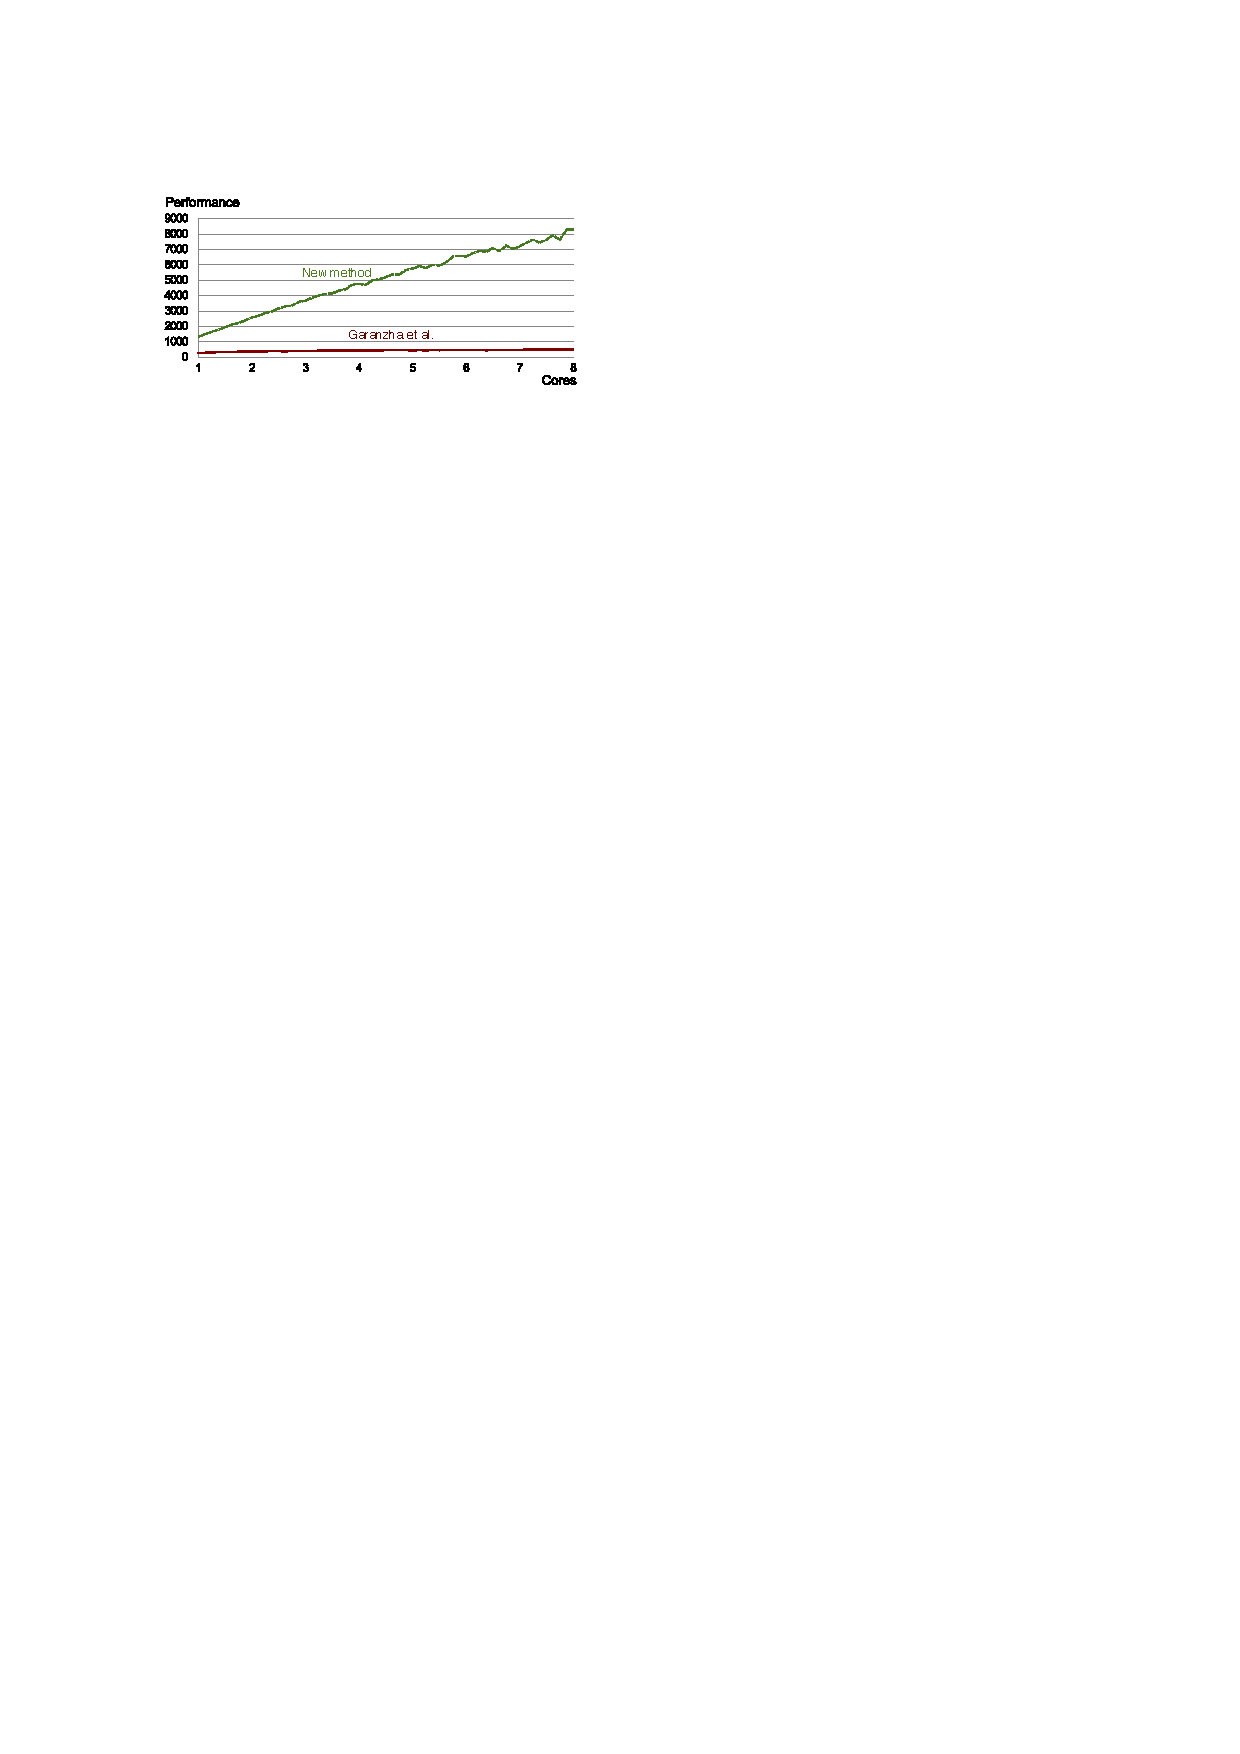
\psfig{file=cores_edited.pdf,width =3in}
\caption{A comparison of two algorithms. The y axis represents millions of primitives per second and the x axis is the number of parallel cores.~\cite{Karras:2012}.}
\label{fig:RadixCores}
\end{figure}

\begin{figure}
\centering
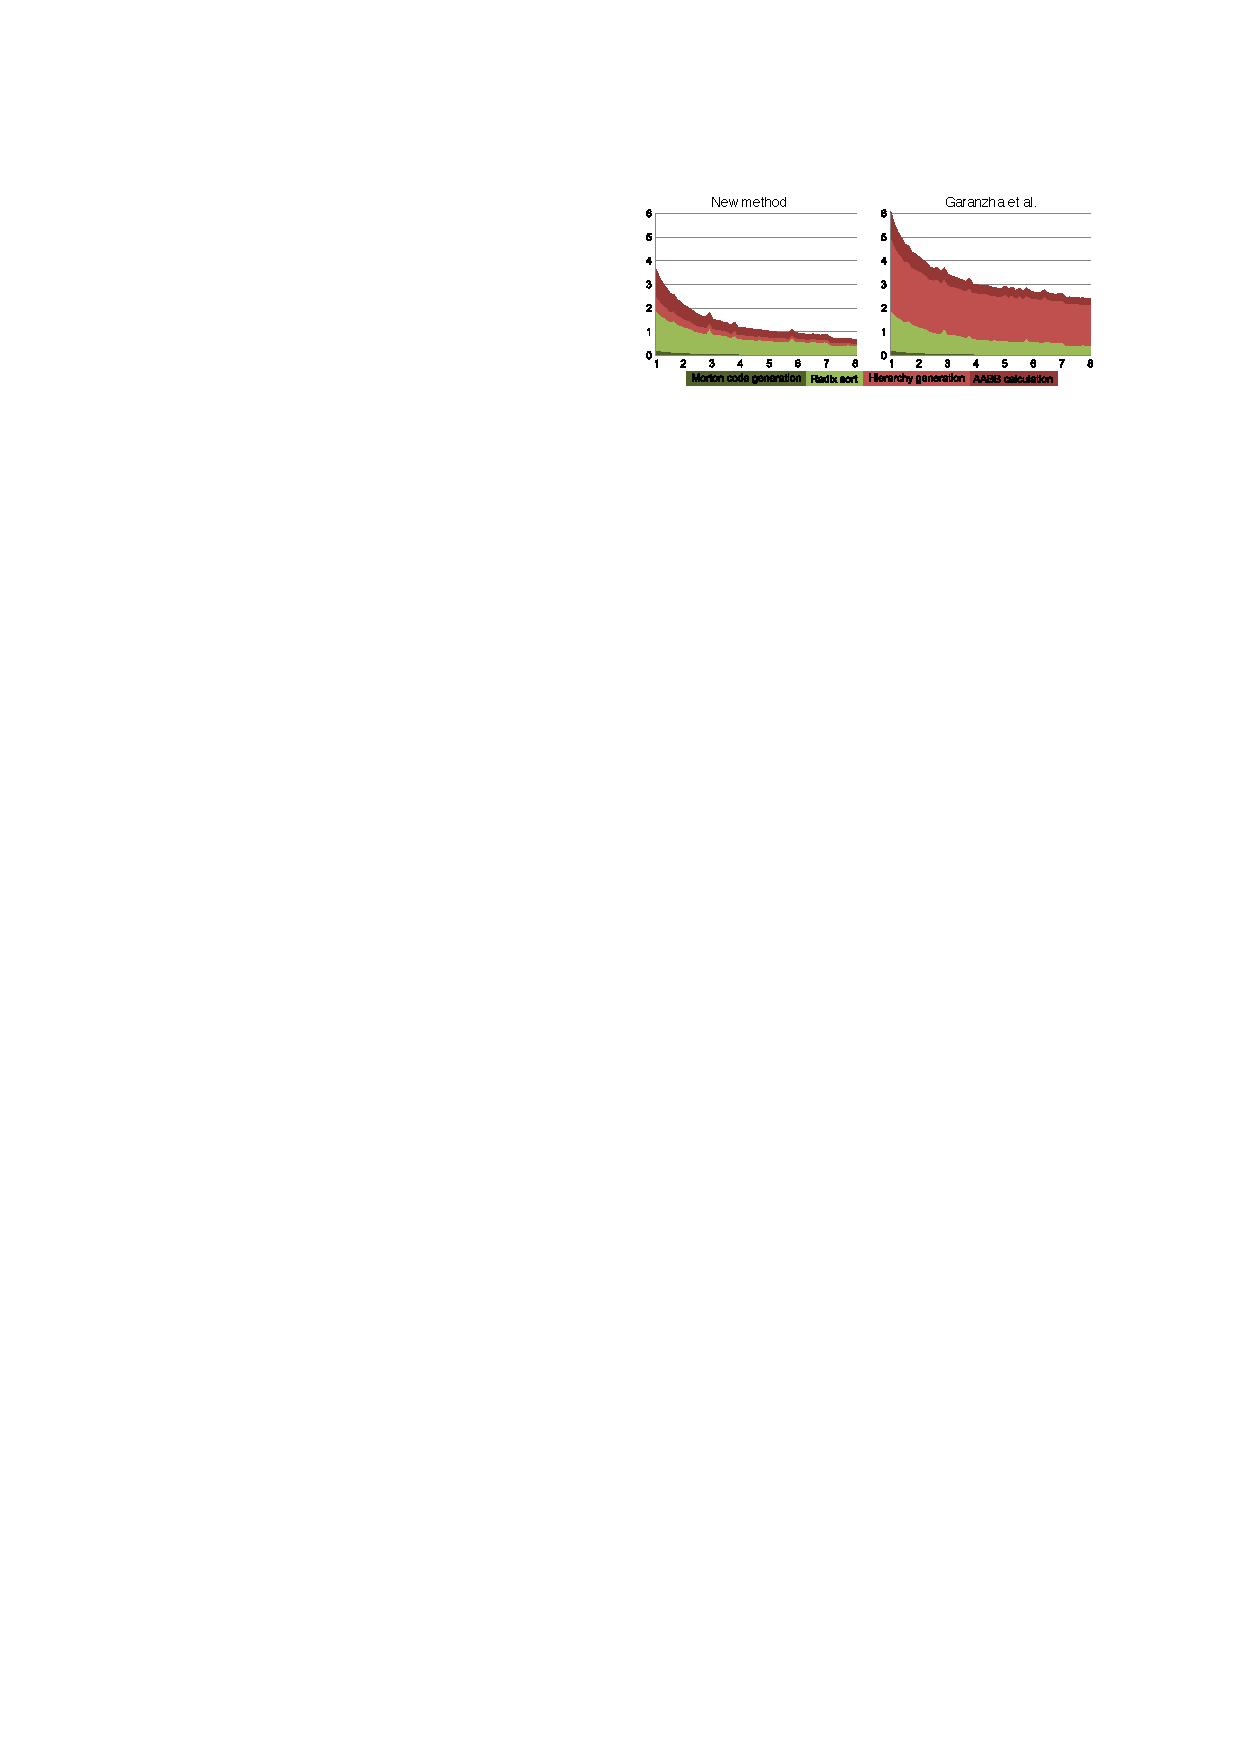
\psfig{file=performance_edited.pdf,width =3in}
\caption{A comparison of two algorithms for constructing a BVH for the Stanford Dragon scene (not shown).~\cite{Karras:2012}.}
\label{fig:RadixPerformance}
\end{figure}

\todo[inline]{Needs more work}

\section*{Acknowledgments}
\label{sec:acknowledgments}

Thanks to Nic McPhee, Elena Machkasova, and Emma Sax for their time, feedback, and constructive comments.

% The following two commands are all you need in the
% initial runs of your .tex file to
% produce the bibliography for the citations in your paper.
\bibliographystyle{abbrv}
% sample_paper.bib is the name of the BibTex file containing the
% bibliography entries. Note that you *don't* include the .bib ending here.
\bibliography{sample_paper}  
% You must have a proper ".bib" file
%  and remember to run:
% latex bibtex latex latex
% to resolve all references

\end{document}
